\chapter{Implementation Design}
\label{ch:implementation}



\section{Design of the Physical Architecture}
\label{sec:phys}

Before I can write the Ansible playbook to deploy the OpenStack cloud, I need to know exactly what I need to deploy. I have designed a basic physical architecture that I will use, and this charpter will describe it.

\subsection{Selecting OpenStack Services}
The first decision when designing an OpenStack cloud deployment is about the services we need to have running.

For this thesis, I have chosen these five core services:
\begin{itemize}
  \item{OpenStack Identity (Keystone)}
  \item{OpenStack Image (Glance)}
  \item{OpenStack Compute (Nova)}
  \item{OpenStack Networking (Neutron)}
  \item{OpenStack Block Storage (Cinder)}
  \item{OpenStack Dashboard (Horizon)}
\end{itemize}

OpenStack consists of several components. I have chosen these six as they are the minimum to have a cloud deployment where I can create virtual machines, attach them to networks, use routers and other networking devices, attach a persistent block storage, and also manage the cloud by a web interface. Implementing more services would be out of the scope of the Thesis.


The services mentioned above will require a database to store their states, and a message broker for some processes to communicate. Specifically, these two services will be needed:
\begin{itemize}
  \item{SQL Database}
  \item{AMQP message broker}
\end{itemize}



\subsection{Selecting Specific Implementations}
The second decision is about the specific implementation of each technology. The OpenStack cloud comes in several releases. The newest release at the time of writing this Thesis is OpenStack Liberty. I will use this relase as I want to develop for the newest stable version available.


I also need to choose an operating system platform that will run on the physical host machines. Choosing the right Linux distribution is important as there might be big differences in terms of available packages, stability, the lifecycle, and an option of commercial support. For this Thesis, I have chosen a CentOS 7.2. CentOS is free and open source operating system based on the Red Hat Enterprise Linux platform. It uses the RPM packaging model and the OpenStack Liberty packages are included in the repositories. The system is stable, has a long lifecycle and potential migration to to a commercially supported environment would be easy, as it is based on the Red Hat Enterprise Linux platform. I have also chose this particular distribution as I know the environment well enough to perform needed configurations and debugging.

OpenStack also needs an SQL database to store the state of the services, and it also might be used as a storage for the Identity service. In this deployment, it will be used in this way. I have chosen MariaDB because it is open source and widely used SQL database. It also comes with the CentOS distribution by default.

The next component is an AMQP broker. It is used by processes within the OpenStack services for communication, and it also might be used as a short-term storage by some networking plugins. For this particular deployment, I will use RabbitMQ because it is an open source solution and it is widely used in production environments. It is also well-supported by the OpenStack itself.

The last decision will be about storage backend for the OpenStack Block Storage service. I will use a local disk and an LVM technology. LVM is a robust and stable open source solution for storage that runs on commodity hardware, which is important especially for this testing environment.


\subsection{Physical architecture}

With the knowledge of the specific components and their implementations, I can design a physical architecture of the deployment I will be using in this Thesis. The physical architecture can be seen on picture \ref{fig:openstack_physical_arch}. It consists of three hosts, referred to as nodes. The description of the nodes is as follows:

\subsubsection{Controller node}
The controller node is the central point of this OpenStack architecture. It will controll and command the whole cloud, and it will also store the state of the cloud. It will host both of the external services: MariaDB and RabbitMQ. There will be also the controller parts of the Compute and Block Storage services. To make this setup easier, it will also host the whole Networking service. However, in large production deployments, the Networking service might be installed on a separate node.

The communication between all OpenStack services will go trough this node, as it also hosts the Identity service that will act as an API. Also, the Dashboard service will be deployed to this nodes. The administrators and the end users will be accessing the cloud via the controller node.

\subsubsection{Compute node}

The compute node will host the Nova Compute service and will act as a hypervisor. All instances in the cloud will run on this node. It is designed in a way it can scale horizontally in need of extra resources. It means that there can be serveral compute nodes deployed at the same time. If this happends, the Nova scheduler service deployed on the controller node will automatically choose the most suitable compute node for all new virtual machines.

\subsubsection{Storage node}

The storage node will provide persistent storage to the virtual machines. It has been separated so the storage can scale independently of the compute resources and vice versa. The storage node is designed in a way that it can scale horizontally, in the same way as the compute node which means that there can be more storage nodes deployed at the same time.


\begin{figure}[!h]
  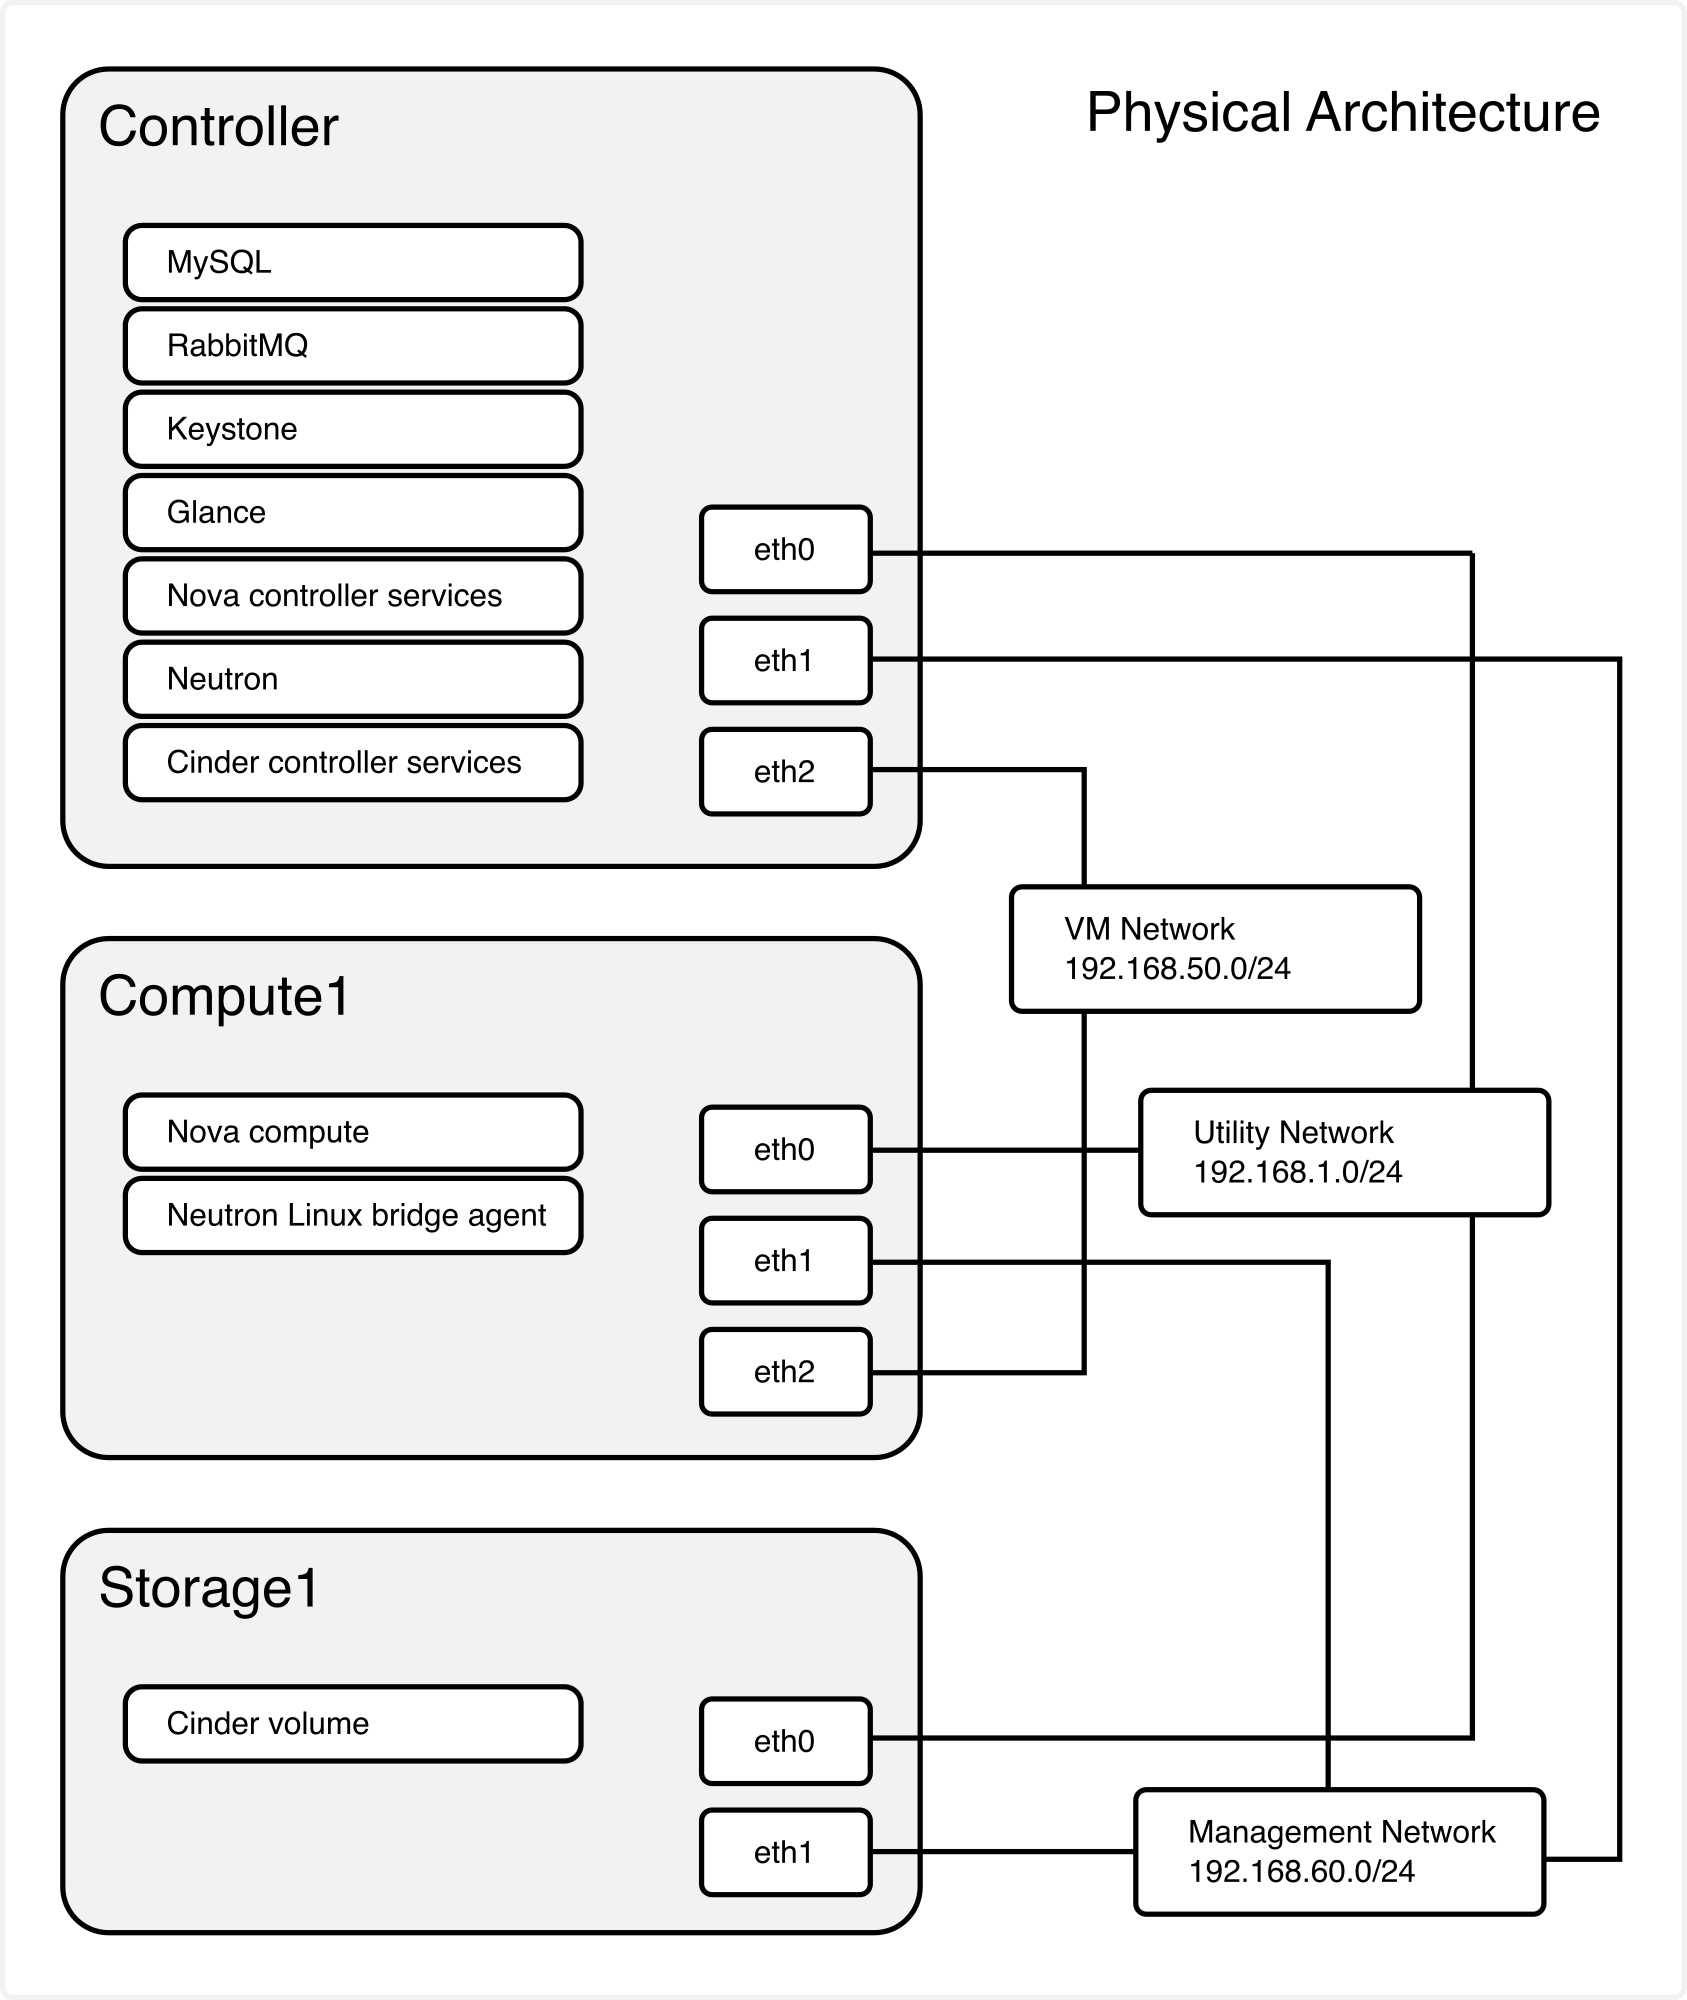
\includegraphics[width=\textwidth]{fig/my_architecture.png}
  \caption{OpenStack physical architecture design}
  \label{fig:openstack_physical_arch}
\end{figure}

\subsubsection*{Networks}
I have used three different networks in my architecture and each one have different purpose in the whole system. Their descriptions are as follows:
\begin{itemize}
  \item{\textbf{Utility Network} - This network is used the datacenter administrators to maintain the physical hosts. In this example it will also be used by Ansible to deploy the OpenStack and all other services.}
  \item{\textbf{Management Network} - This network is used by the OpenStack services to communicate with each other. It will also provide connectivity for the services to the MySQL database and the RabbitMQ Message Queue. All Keystone endpoints based on hostnames will also use this network. It will be also used to connect storage from Storage1 host to virtual machines running on the Compute1 host.}
  \item{\textbf{VM Network} - This network is used to provide outside connectivity to the virtual machines running on the compute node.}
\end{itemize}

There is a separate Utility and Management network. This is because the IP adresses on the Management network are setted up during the deployment. These two networks can be joined together if the IP adresses are properly set before and will not change during deployment. This information might be important when testing on physical nodes with limited number of network connectors.

It is also important to note that the eth2 interfaces on Controller and Compute1 hosts will use special configuration without an IP address and will be attached to virtual network bridges. Their specific configuration will be mentioned later in the text.


\section{Design of the Ansible Playbook}

The Ansible playbook will be designed in a way that it will deploy the physical architecture designed above. To achieve this, it will require minimal configuration, such as IP addresses, hostnames, and passwords - so the level of abstraction will be high enough for the administrator to deploy OpenStack without deep knowledge about it as they will only need to know the IP adresses, hostnames, and passwords.

However, the real benefit of this playbook will be in the reusability for different architectures. In addition of configuring the basic options mentioned above, it will be possible to change the script itself to match other architectures. To make this as easy as possible, I will use the minimal level of abstraction when writing the playbook. I will only use the most basic operations such as installing specific packages using yum, changing the OpenStack configuration files, and restarting systemd services. This minimal abstraction will allow to make much more customisations of the playbook than it is possible to do with Packstack. However, it will require much deeper understanding of the OpenStack architecture which might make it harder to use for some people.

\subsection{Ansible Roles}
The services will be installed on the target hosts using Ansible roles. Roles offer flexibility in a way, that each role can be installed separately on a given host, or, if needed, on multiple hosts. These roles can be then reused to deploy a different physical architectures.

All roles use handlers to restart services in case of a configuration change. All roles are also designed to be idempotent.

There is a role for each OpenStack service. Some services, such as OpenStack Compute and OpenStack Block Storage, will be divided into two roles: the controller part, installed on the controller node, and the functional part, installed on respective nodes.

There will be two other roles to install the database and the AMQP message bus.

Following is the description of each indivitual role.

\subsubsection*{Role \texttt{sql-database}}
The role sql-database will deploy a MariaDB database on the target host. It will set the root password accordingly and will also remove the anonymous user as well as the test database.

The following packages will be installed:
\begin{itemize}
\item{\texttt{mariadb}}
\item{\texttt{mariadb-server}}
\item{\texttt{MySQL-python}}
\end{itemize}

And the following MariaDB service will be enabled and started:
\begin{itemize}
\item{\texttt{mariadb}}
\end{itemize}

\subsubsection*{Role \texttt{rabbit}}
The rabbit role will deploy a RabbitMQ message broker on the target host. It will also create a new user needed for the OpenStack deployment.

The following package will be installed:
\begin{itemize}
  \item{\texttt{rabbitmq-server}}
\end{itemize}

And the following RabbitMQ service will be enabled and started:
\begin{itemize}
  \item{\texttt{rabbitmq-server}}
\end{itemize}

\subsubsection*{Roles \texttt{controller-basic} and \texttt{compute-basic}}
The roles controller-basic and compute-basic enable the OpenStack Liberty repository for CentOS and install the SELinux package. These roles are the first that should be run before any other openstack roles.

These roles will install these two packages:
\begin{itemize}
  \item{\texttt{python-openstackclient}}
  \item{\texttt{openstack-selinux}}
\end{itemize}

\subsubsection*{Role \texttt{keystone}}
The keystone role will install the OpenStack Identity service, codename Keystone, on the target host. It requires an SQL database to be running on the network. The design used in this thesis will run the database on the controller node.

The role will create a database for the Keystone service called keystone.

This role will install the following packages:
\begin{itemize}
  \item{\texttt{openstack-keystone}}
  \item{\texttt{httpd}}
  \item{\texttt{mod\_wsgi}}
  \item{\texttt{memcached}}
  \item{\texttt{python-memcached}}
  \item{\texttt{python-keystoneclient}}
\end{itemize}
And it will enable and start the httpd service on the target host.



\subsubsection*{Role \texttt{glance}}
The glance role will install the OpenStack Image service, codename Glance, on the target host. It requires an SQL database, and the OpenStack Identity service to be running on the network. The example in this thesis will run both on the controller node.

The role will create a database for the Glance service called glance, and registers the Glance service and creates endpoints in the Keystone service.

Glance supports several backends for storing images. This role uses local filesystem to do so. Metadata about the images will be stored in the SQL database running on the controller node.

This role will install the following packages:
\begin{itemize}
  \item{\texttt{openstack-glance}}
  \item{\texttt{python-glance}}
  \item{\texttt{python-glanceclient}}
\end{itemize}
And the two following services will be enabled and started:
\begin{itemize}
  \item{\texttt{openstack-glance-api}}
  \item{\texttt{openstack-glance-registry}}
\end{itemize}


\subsubsection*{Role \texttt{nova-controller}}
The nova-controller role will install some parts of the OpenStack Compute service, codename Nova, on the target host. It requires an SQL database, RabbitMQ message bus, and the OpenStack Identity service to be running on the network. The example in this thesis will run all these services on the controller node.

The role will create a database for the Nova service called nova, and registers the Nova service and creates endpoints in the Keystone service.

Besides the standard configurations such as setting hostname, configuration of database, and message bus access, the Nova service will be configured to use the OpenStack Networking (as opposed to legacy Nova networking) with the Linux bridge driver.

This role will install the following packages:
\begin{itemize}
  \item{\texttt{openstack-nova-api}}
  \item{\texttt{openstack-nova-cert}}
  \item{\texttt{openstack-nova-conductor}}
  \item{\texttt{openstack-nova-console}}
  \item{\texttt{openstack-nova-novncproxy}}
  \item{\texttt{openstack-nova-scheduler}}
  \item{\texttt{python-novaclient}}
\end{itemize}
And the following services will be enabled and started:
\begin{itemize}
  \item{\texttt{openstack-nova-api}}
  \item{\texttt{openstack-nova-cert}}
  \item{\texttt{openstack-nova-consoleauth}}
  \item{\texttt{openstack-nova-scheduler}}
  \item{\texttt{openstack-nova-conductor}}
  \item{\texttt{openstack-nova-novncproxy}}
\end{itemize}

\subsubsection*{Role \texttt{nova-compute}}
The nova-compute role will install the nova-compute process of the OpenStack Compute service, codename Nova, on the target host. It requires the RabbitMQ message bus to be running on the network. The example in this thesis will run it on the controller node.

The role will configure an access to the necessary Nova processes installed by the nova-controller role, and will also configure Nova to use the OpenStack Networking with the Linux bridge driver.

It will also configure the hypervisor. This role uses the libvirt provider with QEMU. This is because VirtualBox, which is used for testing the deployment, does not support nested virtualisation, so KVM can not be used.

This role will install these two packages:
\begin{itemize}
  \item{\texttt{openstack-nova-compute}}
  \item{\texttt{sysfsutils}}
\end{itemize}
And will start and enable the two following services:
\begin{itemize}
  \item{\texttt{libvirtd}}
  \item{\texttt{openstack-nova-compute}}
\end{itemize}

\subsubsection*{Role \texttt{neutron-controller}}
The neutron-controller role will install the OpenStack Networking service, codename Neutron, on the target host. It requires an SQL database, RabbitMQ message bus, and the OpenStack Identity service to be running on the network. The example in this thesis will run all these services on the controller node. This role also requires the nova-compute role to be run on the same host before.

The role will create a database for the Neutron service called neutron, and registers the Neutron service and creates endpoints in the Keystone service.

The OpenStack Networking service uses plug-ins and agents for the actual networking functionality. This role will use:
\begin{itemize}
  \item{\texttt{Modular Layer 2 (ML2) plugin}}
  \item{\texttt{Linux bridge agent}}
  \item{\texttt{Layer-3 agent}}
  \item{\texttt{DHCP agent}}
\end{itemize}
This setup will allow to create tenant networks as well as public provider networks.

The ML2 plugin will be configured to use the Linux bridge technology and VXLAN to create the tenant networks. The Linux bridge agent will be configured to use VXLAN for the tenant networks and iptables firewall driver to manage security groups. The layer-3 agent will be configured to use the Linux bridge driver and to support multiple external networks.

The DHCP agent will be also configured to use the Linux bridge driver and the MTU is set to 1450 bytes. This is because the VXLAN includes additional packet header and virtual machines running in the cloud use the default MTU of 1500 bytes. Using this settings, the virtual machines will use the smaller MTU, which would allow space for the additional header.

Finally, the Nova service will be configured to use the OpenStack Networking service, installed by this role.

This role will install the following packages:
\begin{itemize}
  \item{\texttt{openstack-neutron}}
  \item{\texttt{openstack-neutron-ml2}}
  \item{\texttt{openstack-neutron-linuxbridge}}
  \item{\texttt{python-neutronclient}}
  \item{\texttt{ebtables}}
  \item{\texttt{ipset}}
\end{itemize}
It will restart this service:
\begin{itemize}
  \item{\texttt{openstack-nova-api}}
\end{itemize}
And the following services will be started and enabled:
\begin{itemize}
  \item{\texttt{neutron-server}}
  \item{\texttt{neutron-linuxbridge-agent}}
  \item{\texttt{neutron-dhcp-agent}}
  \item{\texttt{neutron-metadata-agent}}
  \item{\texttt{neutron-l3-agent}}
\end{itemize}


\subsubsection*{Role \texttt{neutron-compute}}
The neutron-compute role will install the Linux bridge agent of the OpenStack Networking service, codename Neutron, on the target host.  It requires the RabbitMQ message bus to be running on the network. The example in this thesis will run it on the controller node. It also require the role nova-compute to be run on the same host before.

This role will configure the Linux bridge agent to use the correct network interface as a public interface, enables VXLAN for the tenant networks, and configures iptables as a firewall driver to manage security groups.

It will also configure the Nova service to use the OpenStack Networking.

This role will install the following packages:
\begin{itemize}
  \item{\texttt{openstack-neutron}}
  \item{\texttt{openstack-neutron-linuxbridge}}
  \item{\texttt{ebtables}}
  \item{\texttt{ipset}}
\end{itemize}
It will restart this Nova service:
\begin{itemize}
  \item{\texttt{openstack-nova-compute}}
\end{itemize}
And also the Linux bridge agent service will be started and enabled:
\begin{itemize}
  \item{\texttt{neutron-linuxbridge-agent}}
\end{itemize}



\subsubsection*{Role \texttt{cinder-controller}}

The cinder-controller role will install the OpenStack Block Storage service, codename Cinder, on the target host. It requires an SQL database, RabbitMQ message bus, and the OpenStack Identity service to be running on the network. The example in this thesis will run all these services on the controller node.

The role will create a database for the Cinder service called cinder, and registers two services called \textit{cinder} and \textit{cinderv2}, and creates endpoints for each service. Two services are created, because the OpenStack Block Storage service currently supports two versions of API. This role will use both for better compatibility.

The following packages will be installed:

\begin{itemize}
  \item{\texttt{openstack-cinder}}
  \item{\texttt{python-cinderclient}}
\end{itemize}

The \texttt{openstack-nova-api} service needs to be restarted first, and then the following services will be enabled and started:
\begin{itemize}
  \item{\texttt{openstack-cinder-api}}
  \item{\texttt{openstack-cinder-scheduler}}
\end{itemize}


\subsubsection*{Role \texttt{cinder-storage}}

This cinder-storage role will install the storage part of the OpenStack Block Storage service, codename Cinder, on the target host. It requires the RabbitMQ message bus to be running on the network. The example in this thesis will run it on the controller node.

At first, the role makes sure that there is a partition available for the storage, and creates an LVM volume group. Then it configures the Block Storage service to use this volume group to create individual volumes of persistent storage for the virtual machines.

The following packages will be installed:

\begin{itemize}
  \item{\texttt{lvm2}}
  \item{\texttt{openstack-cinder}}
  \item{\texttt{targetcli}}
  \item{\texttt{python-oslo-policy}}
\end{itemize}

And the following services will be started and enabled:

\begin{itemize}
  \item{\texttt{openstack-cinder-volume}}
  \item{\texttt{target}}
\end{itemize}



\subsubsection*{Role \texttt{dashboard}}
The dashboard role will install the OpenStack Dashboard service, codename Horizon, on the target host. The Dashboard service installed by this role uses the Apache httpd web server.

It will install the following packages:
\begin{itemize}
  \item{\texttt{openstack-dashboard}}
  \item{\texttt{httpd}}
  \item{\texttt{memcached}}
\end{itemize}
And the following services will be started and enabled:
\begin{itemize}
  \item{\texttt{httpd}}
  \item{\texttt{memcached}}
\end{itemize}




\subsection{Applying Roles to the Hosts}

The main Ansible playbook will apply the roles designed above to particular hosts. See the table \ref{table-roles} for reference about what roles will be applied to which hosts.

Each role will require several parametres such as IP addresses, hostnames, or passwords to be set. This can be also done in the main playbook.

\begin{table}[!h]
  \centering
  \begin{tabular}{|l|l|}
    \hline
      Host Name       & Applied Roles                             \\
    \hline
    \multirow{9}{*}{Controller node} & \texttt{controller-basic}  \\
      & \texttt{rabbit} \\
      & \texttt{sql-database} \\
      & \texttt{dashboard} \\
      & \texttt{glance} \\
      & \texttt{keystone} \\
      & \texttt{neutron-controller} \\
      & \texttt{nova-controller} \\
      & \texttt{cinder-controller} \\
    \hline
    \multirow{3}{*}{Compute node} & \texttt{compute-basic} \\
      & \texttt{neutron-compute} \\
      & \texttt{nova-compute} \\
      \hline
    \multirow{2}{*}{Storage node} & \texttt{storage-basic} \\
      & \texttt{cinder-storage} \\
    \hline
  \end{tabular}
\caption{Roles applied to the particular hosts}
\label{table-roles}
\end{table}
